\section{Heading from a Recorded Inertial Sensor}
\label{sec:imu}

The heading of a moving sensor is a cyclic state with a continuous position. A
gyroscope measures a noisy increment of this state at every step, while a
magnetometer acts as a pointer reading that magnetic disturbances can corrupt. We
test both cases on BROAD, a public benchmark of 39 trials recorded with an
inertial measurement unit (IMU) and optical motion capture
\citep{laidig2021broad}. The motion capture provides only the labels and never
enters a model input. The protocol was fixed before training, and Appendix~\ref{app:imu}
records every later amendment.

\begin{figure}[!t]
\centering
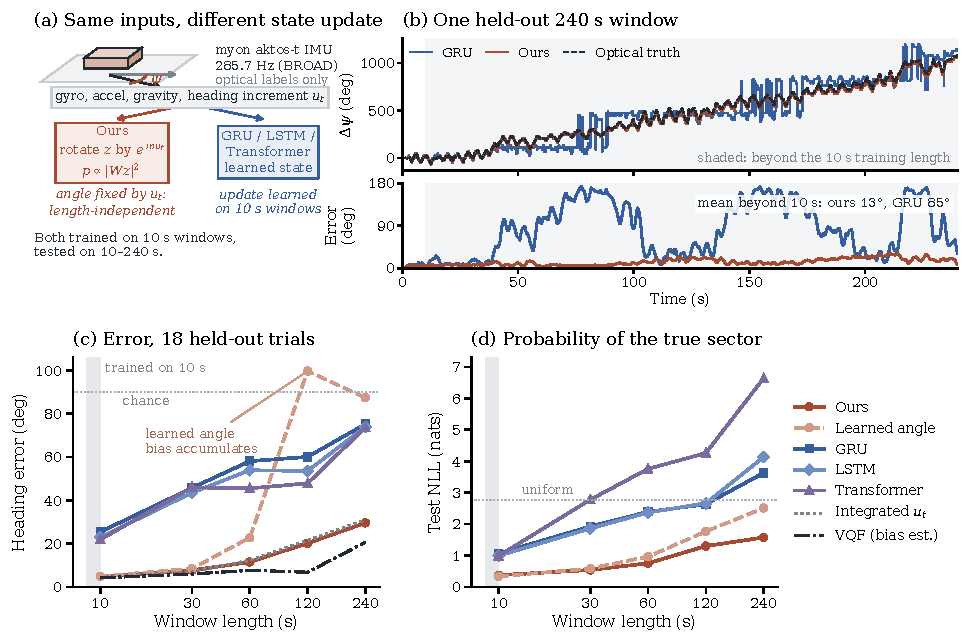
\includegraphics[width=\linewidth]{figures/imu_main.pdf}
\caption{Heading from a recorded IMU (BROAD, myon aktos-t at 285.7~Hz;
\citealp{laidig2021broad}). (a)~All learned models receive the same inputs; ours
sets its rotation angle from the measured increment $u_t$, while the GRU, LSTM,
and Transformer learn their state update. Every model trains on 10~s windows.
(b)~A held-out 240~s window from trial~20 (seed~0): heading change of each
model's most probable sector against the optical truth, and the error (2~s moving
average). (c)~Error at the window end and (d)~test NLL on 18 held-out trials,
averaged over five seeds and then trials. Gray curves are classical filters and
have no NLL. The 240~s windows come from the three longest test trials.}
\label{fig:imu}
\label{fig:imu-sensor}
\end{figure}

\subsection{Observed increments: gyroscope heading}
\label{sec:imu-gyro}
The first task is to estimate the heading change since the start of a window,
binned into 16 sectors of $22.5^\circ$. At 28.6~Hz, every learned model receives
the same inputs (Figure~\ref{fig:imu}a): the gyroscope and accelerometer readings, the gravity direction
from a causal complementary filter \citep{mahony2008complementary}, and that
filter's heading increment $u_t$. Models train on 10~s windows from 18 trials and
are tested on windows of 10 to 240~s from 18 other trials. In our model the input
sets the rotation angle, $\theta_t=n\,u_t$ for harmonics $n=1,\dots,8$, and a Born
readout (Equation~\eqref{eq:born}) turns the rotated state into sector
probabilities; only the readout and the initial phase are learned. A second
variant also learns a correction to the angle. The GRU, LSTM, and Transformer use
the same input encoder and more parameters.

Figure~\ref{fig:imu} summarizes the results. Panel~(b) shows one held-out
window: past the 10~s training length, our model keeps following the optical
heading, while the GRU repeatedly loses it by up to $180^\circ$. Across all test
trials (panels c and d), at every window length the input-set rotation has the lowest error and NLL of all learned models. At 240~s
its heading error is $29.6^\circ$, against $73.7^\circ$ for the best recurrent or
attention model, a paired difference of $-44.1^\circ$ with trial-bootstrap
interval $[-65.5,-31.4]$; the intervals exclude zero at all five lengths for both
error and NLL. The variant with a learned angle correction keeps pace up to 30~s
and then drifts. Its mean correction of $4.4\times10^{-4}$~rad per step is too
small to identify from 10~s windows, yet it accumulates to about $87^\circ$ at
120~s, consistent with the linear growth of angular error bounded in
Section~\ref{sec:stab}. The input-set rotation, in contrast, stays within
$1.4^\circ$ of integrating $u_t$ directly, so it keeps the accuracy of the
physical integrator while adding calibrated sector probabilities. It has no
bias state, however, and VQF, a filter that also estimates gyroscope bias
\citep{laidig2023vqf}, is more accurate from 30~s on and reaches $20.7^\circ$ at
240~s.

\subsection{Pointer readings: magnetometer under disturbance}
\label{sec:imu-mag}
The second task is to estimate the absolute heading in 64 sectors from a uniform
prior, with the tilt-compensated magnetometer heading added at every step as a
pointer reading. Five of the test trials contain recorded magnetic disturbances.
Our cyclic filter (Section~\ref{sec:filter}) shifts a categorical belief by $u_t$
through a phase rotation of its Fourier coefficients and corrects it with a
learned pointer likelihood. Its tracking error matches that of the best neural
network: on disturbed trials at 60~s, the difference from the LSTM is
$-1.4^\circ$ with interval $[-3.4,0.6]$. On undisturbed trials it beats a tuned
complementary filter by $1.2^\circ$ $[-2.1,-0.3]$, but its NLL is higher than that
of the GRU and LSTM. VQF, with its magnetic disturbance rejection, tracks within
$3.4^\circ$ on disturbed trials, against $9.5^\circ$ for our filter, and the
criterion we fixed in advance for this task is not met (Appendix~\ref{app:imu},
Table~\ref{tab:imu-b}).

Both tasks agree with the simulated results. When uncertainty enters through the
increments, fixing the transition to a rotation by the measured increment
generalizes from 10~s to 240~s, and unconstrained sequence models do not. When it
enters through a corrupted pointer, the useful structure lies in the pointer
model: our learned likelihood does not supply it, and the engineered disturbance
rejection in VQF does.
